

\documentclass[compress, xcolor=pst]{beamer}
%\documentclass[compress, xcolor=pst, handout]{beamer}
\usepackage{graphicx}
\graphicspath{ {images/} }
\mode<presentation>
\usepackage{amsfonts, amsmath, amssymb, color}
\useoutertheme{smoothbars}
\usecolortheme{dolphin}
\usecolortheme{rose}
\usepackage{chngpage}
%\usepackage{beamerthemesplit}
\usepackage{lscape}
\usepackage{graphicx}
\usepackage{multirow}
\usepackage{enumerate}
\usepackage{comment}
\usepackage{tikz}
\usetikzlibrary{shapes.geometric, arrows}
\usepackage{multimedia}
\usepackage{empheq}
\usepackage{subcaption}
\usepackage[most]{tcolorbox}

%% === bibliography packages ===
%\usepackage{natbib}
%\bibliographystyle{natbib}

\setbeamertemplate{navigation symbols}{}

\setbeamersize{description width=0.5cm}
\setbeamertemplate{navigation symbols}{}

%\usepackage{spacingset}
\newcommand\spacingset[1]{\renewcommand{\baselinestretch}%
{#1}\small\normalsize}
\newcommand\tab[1][1cm]{\hspace*{#1}}

\usepackage[plain]{algorithm}
\usepackage{algpascal}
\algdef{SE}{For}{End}[2]{%
  \textkeyword{for} \(#1\) \textkeyword{to} \(#2\) }{%
  \textkeyword{end}}
\algdef{SE}{While}{End}[1]{%
  \textkeyword{while} \(#1\)}{%
  \textkeyword{end}}
\algdef{SE}{If}{EndIf}[1]{%
  \textkeyword{if} \(#1\)}{%
  \textkeyword{end}}

\usepackage{color,colortbl}
\DeclareMathOperator*{\argmax}{arg\,max}
\DeclareMathOperator*{\argmin}{arg\,min}


\title{Bayesian Optimization of a Wearable Assistive Device Using an Estimator Stopping Process}
\author[]{Charles Liu\\ \texttt{cliu02@g.harvard.edu}}
\institute{IACS, Harvard University}
\date{May 4, 2018}

\begin{document}

\frame{\titlepage}


\section{Introduction}
\begin{frame}
    \frametitle{\textbf{Soft Exosuit}}
	\movie[loop, autostart, showcontrols, height = 0.6\textwidth, width = \textwidth]{}{IMG_4348.MOV}
\end{frame}

\begin{frame}
    \frametitle{\textbf{Process Overview}}
	\begin{figure}
		\centering
		\scalebox{.75}{\tikzstyle{startstop} = [rectangle, rounded corners, minimum width=3cm, minimum height=1cm,text centered, text width=3cm, draw=black, fill=red!30]
\tikzstyle{process} = [rectangle, minimum width=3cm, minimum height=1cm, text centered, text width=2.5cm, draw=black, fill=orange!30]
\tikzstyle{decision} = [rectangle, minimum width=3cm, minimum height=1cm, text centered, text width=2.5cm, draw=black, fill=green!30]
\tikzstyle{arrow} = [thick,->,>=stealth]
    
\begin{tikzpicture}[node distance=2cm]

\node (measurement) [startstop] {Respiratory Measurement};
\node (estimator) [process, below of=measurement] {Metabolic Estimation (Ch.2)};
\node (stopping) [decision, below of=estimator, yshift=-0.5cm] {Change Parameter Settings? (Ch.3)};
\node (bayesopt) [process, below of=stopping, yshift=-1cm] {Select New Parameter Settings (Ch.1)};

\draw [arrow] (measurement) -- (estimator);
\draw [arrow] (estimator) -- (stopping);
\draw [arrow] (stopping) --++ (3cm,0cm) |- node[anchor=west, yshift=-2cm] {no} (measurement);
\draw [arrow] (stopping) -- node[anchor=east] {yes} (bayesopt);
\draw [arrow] (bayesopt) --++ (-3cm,0cm) |- (measurement);


\end{tikzpicture}}
	\end{figure}
\end{frame}

\section{Parameter Selection}
\begin{frame}
	\frametitle{\textbf{Standard Gaussian Process Model}}
	Observations represent underlying process with some Gaussian noise
	\begin{align*}
		y &\sim f + \mathcal{N}(0, \sigma_n^2)\\
		f &\sim \mathbb{G}(0, \kappa)\\
		\kappa(x_i, x_j \vert \sigma_\theta^2, l) &= \sigma_\theta^2 \exp(-\frac{1}{2}d^2(\frac{x_i}{l}, \frac{x_j}{l}))
	\end{align*}
\end{frame}

\begin{frame}
	\frametitle{\textbf{Gaussian Process Regression}}
	Given some training data, closed form posterior distribution at any point $x$
	\begin{gather*}
	  \bar{\mu}(x) = K(X, x)^T[K(X, X) + \sigma_n^2 I]^{-1}Y \\
	  \bar{\sigma}^2(x) = \kappa(x, x\vert \theta) - K(X, x)^T[K(X,X) + \sigma_n^2 I]^{-1}K(X,x) \\
	  K(X,x)_i = \kappa(x_i, x\vert \theta)\\
	  K(X,X)_{ij} = \kappa(x_i, x_j\vert \theta),
	\end{gather*}
	where $X = \{x_i\}_{i=1}^n$ and $Y = \{y_i\}_{i=1}^n$. 
\end{frame}

\begin{frame}
	\frametitle{\textbf{$\sigma_\theta^2$ Effect}}
	\begin{figure}
	\centering
	\includegraphics[width=\textwidth]{magn_regression}
	\end{figure}
\end{frame}

\begin{frame}
	\frametitle{\textbf{Hyperparameter Estimation}}
	\begin{figure}
	\centering
	\includegraphics[width=\textwidth]{hyperparamprob.png}
	\end{figure}
\end{frame}

\begin{frame}
	\frametitle{\textbf{Expected Improvement}}
	\begin{align*}
	  EI(x\vert \mathbb{S}) &= \int_\infty^\infty max(0, y^*-y)p(y\vert x)dy\\
	    &= z\bar{\sigma}(x)\Phi(z) + \bar{\sigma}(x)\phi(z)\\
	  z &= \frac{y^* - \bar{\mu}(x) + \xi}{\bar{\sigma}(x)},
	\end{align*}
	where $y^*$ is the best value observed so far, $\Phi(z)$ and $\phi(z)$ are the standard normal CDF and PDF functions, and $\xi$ is a scaling parameter to adjust the tradeoff between exploration-exploitation
\end{frame}

\begin{frame}
	\frametitle{\textbf{Bayesian Optimization}}
	\begin{algorithmic}
	\State \textkeyword{Objective Function} $F(x)$
	\State \textkeyword{Acquisition Function} $g(\mu, \sigma^2)$
	\State \textkeyword{Specify Exploration Points } $\mathbb{E} = \{e_1, e_2, ..., e_n\}$
	\State \textkeyword{Training Samples } $\mathbb{S}$
	\For{i=1}{n}
	  \State $\mathbb{S} = \mathbb{S} \cup \{e_i, F(e_i)\}$
	\End
	\While{t < T}
	  \State Update GP Hyperparameters $\theta$
	  \State Given $f(x\vert \theta, \mathbb{S}) \sim \mathcal{N}(\mu_x, \sigma_x^2)$,
	  \State $x^* = \argmax_{x \in \mathbb{X}} g(\mu_x, \sigma_x^2)$
	  \State $\mathbb{S} = \mathbb{S} \cup \{x^*, F(x^*)\}$
	\End
	\end{algorithmic}
\end{frame}

\section{Metabolic Estimation}
\begin{frame}
	\frametitle{\textbf{Instantaneous Energetic Cost}}
	\begin{figure}
	\centering
	\includegraphics[width=\textwidth]{metabolicestimation.png}
	\end{figure}
\end{frame}

\begin{frame}
	\frametitle{\textbf{Kalman Filter}}
	System Dynamics
	\begin{align*}
	  x(t+1) &= F(x(t), v(t), t)\\
	  z(t) &= H(x(t), w(t), t)\\
	\end{align*}

	Update Equations
	\begin{align*}
	  \hat{x}(t) &= \hat{x}(t\vert t-1) + Ky \\
	  P_{x}(t) &= P_{x}(t\vert t-1) - KP_{y}(t\vert t-1) K^T\\
	  K &= P_{xy}(t\vert t-1) P_{y}^{-1}(t\vert t-1)\\
	  y &= z(t) - H(\hat{x}(t\vert t-1) , w(t), t)
	\end{align*}
\end{frame}

\begin{frame}
	\frametitle{\textbf{Unscented Transform}}
	\vspace{-2em}
	\begin{align*}
	  \chi_0 &= \bar{x}\\
	  \chi_i &= \bar{x} + (\sqrt{(N + \lambda)P_x})_i & i = 1, ..., N \\
	  \chi_i &= \bar{x} - (\sqrt{(N + \lambda)P_x})_{i-N} & i = N + 1, ..., 2N\\
	  W_0^{(m)} &= \lambda /(N + \lambda) \\
	  W_0^{(c)} &= \lambda /(N + \lambda) + (1- \alpha^2 + \beta)\\
	  W_i^m &= W_i^c = 1/\{(2(N + \lambda))\} & i = 1, ..., 2N,
	\end{align*}
	where $\lambda = \alpha^2(N + \kappa) - N$, and $\alpha$, $\kappa$, and $\beta$ are scaling parameters. Given $y=g(x)$,
	\begin{align*}
	  \bar{y} &\approx \sum_{i=0}^{2N} W_i^{(m)}g(\chi_i)\\
	  P_y &\approx \sum_{i=0}^{2N} W_i^{(c)}(g(\chi_i) - \bar{y})(g(\chi_i) - \bar{y})^T
	\end{align*}
\end{frame}

\begin{frame}
	\frametitle{\textbf{UKF Model}}
	Time constants $\tau_0, \tau$ characterizing rate of change of cost constants $c_0, c$
	\begin{align*}
		x &= [c_0 \text{ } c \text{ } \tau_0 \text{ } \tau]\\
	    F(x(t), v(t), t) &= x(t) + v(t)\\
	    H(x(t), w(t), t) &= c(1-e^{\frac{-t}{\tau}}) + c_0e^{\frac{-t}{\tau_0}} + w(t)
	\end{align*}
\end{frame}

\begin{frame}
	\frametitle{\textbf{Measurement Noise}}
	\begin{figure}
	\centering
	\includegraphics[width=\textwidth]{measurementnoise.png}
	\end{figure}
\end{frame}

\begin{frame}
	\frametitle{\textbf{Estimator in Subject Trials}}
	\begin{figure}[t]
	\centering
	
\includegraphics[width=\textwidth]{subjcostest.png}
	\end{figure}
\end{frame}

\section{Stopping Models}
\begin{frame}
	\frametitle{\textbf{Stopping Problem Formulation}}
	\begin{table}
		\centering
		\begin{tabular}{ |c  c| }
		  \hline&\\
		  $N$ & Finite horizon\\
		  &\\
		  $X_t$ & State at time $t$\\
		  &\\
		  $P(X_t \vert X_{t-1})$ & State transitions, typically Markovian\\
		  &\\
		  $\lambda$ & Discount Factor $\in (0, 1]$\\
		  &\\
		  $r(X)$ & Bounded reward function for continuing at state $X$\\
		  &\\
		  $g(X)$ & Bounded reward function for stopping at state $X$\\
		  &\\
		  \hline
		\end{tabular}
		\end{table}
\end{frame}

\begin{frame}
	\frametitle{\textbf{Optimal Stopping Point}}
	Via backward induction
	\begin{align*}
	  J_N(x) &= g(x)\\
	  J_n(x) &= max\{g(x), r(x) + \lambda\mathbb{E}_{P(y\vert x)}[J_{n+1}(y)]\}
	\end{align*}
	Optimal stopping point
	\begin{align*}
	  \tau = \min_{t}J_t(X_t) = g(X_t)
	\end{align*}
\end{frame}

\begin{frame}
	\frametitle{\textbf{Distribution of Interest}}
	Given
	\begin{align*}
		\text{Current Estimate: } \hat{x}_t &\sim \mathcal{N}(\mu_{x_t}, \sigma^2_{x_t})\\
		\text{Best Estimate: } \hat{x}^* &\sim \mathcal{N}(\mu_{x^*}, \sigma^2_{x^*})
	\end{align*}
	We are concerned with
	\begin{align*}
	    \hat{x}_t - \hat{x}^* &\sim \mathcal{N}(\mu, \sigma^2)\\
	    \mu &= \mu_{x_t} - \mu_{x^*}\\
	    \sigma^2 &= \sigma^2_{x_t} + \sigma^2_{x^*}
	\end{align*}
\end{frame}

\begin{frame}
	\frametitle{\textbf{$\sigma$-Offset Model}}
	\begin{align*}
	  X_t &= \mu\\
	  P(X_t \vert X_{t-1}) &= P(X_t) \sim \mathcal{N}(\mu, \sigma^2)\\
	  r(x) &= K\sigma-x\\
	  g(x) &= 0
	\end{align*}
	Stopping condition $X_t > K\sigma$
\end{frame}

\begin{frame}
	\frametitle{\textbf{Success/Failure Model}}
	Define success as
	\begin{align*}
		\Phi(\frac{\mu}{\sigma}) > K,
	\end{align*}
	for risk tolerance $K$. Define model as
	\begin{align*}
	  X_t &= (\alpha_t + \alpha_0, \beta_t + \beta_0) \\
	  P(X_{t+1}) &=
	  \begin{cases}
	      (\alpha_t + \alpha_0 + 1, \beta_t + \beta_0)
	      \\ \tab\text{w.p. } \frac{\alpha_t + \alpha_0}{\alpha_t + \alpha_0 + \beta_t + \beta_0}\\
	      (\alpha_t + \alpha_0, \beta_t + \beta_0 + 1)
	      \\ \tab\text{w.p. } \frac{\beta_t + \beta_0}{\alpha_t + \alpha_0 + \beta_t + \beta_0}
	  \end{cases}\\
	  r(X_t) &= \frac{\alpha_t + \alpha_0}{\alpha_t + \alpha_0 + \beta_t + \beta_0},
	\end{align*}
	with smoothing priors $\alpha_0,\beta_0$ and success/failures $\alpha_t,\beta_t$
\end{frame}

\begin{frame}
	\frametitle{\textbf{Multi-Armed Bandit Problem}}
	Which is the better option?
	\begin{itemize}
		\item Option 1: 20 successes, 20 failures
		\item Option 2: 3 successes, 4 failures
	\end{itemize}
	Assume $g(x) = g$ is a constant, define Gittins Index as
	\begin{gather*}
	  \nu(X_t) = (1-\lambda)\min_{g} \{J_t(X_t) = g\}\\
	  \nu((30, 30)) = 0.5133
	\end{gather*}
	\begin{empheq}[box=\tcbhighmath]{equation*}
		\nu((4, 6)) = 0.5289
	\end{empheq}

	In the case of single option, must set another threshold $\nu(x) < V$
\end{frame}

\begin{frame}
	\frametitle{\textbf{Adaptive Threshold}}
	Use the exploration phase of Bayesian optimization to tune thresholds in either model, with final distribution for each point as "best" value. Consider a window of values at time $t$
	\begin{table}
    \centering
    \begin{tabular}{|c|c|>{\columncolor[gray]{0.8}}c|>{\columncolor[gray]{0.8}}c|>{\columncolor[gray]{0.8}}c|c|c|c|c|c}
        \hline
        $e_{00}$&$e_{01}$&$e_{02}$&$e_{03}$&$e_{04}$&$e_{05}$&$e_{06}$&$e_{07}$&$e_{08}$&$e_{09}$\\\hline
        $e_{10}$&$e_{11}$&$e_{12}$&$e_{13}$&$e_{14}$&$e_{15}$&$e_{16}$&$e_{17}$&$e_{18}$&$e_{19}$\\\hline
        $e_{20}$&$e_{21}$&$e_{22}$&$e_{23}$&$e_{24}$&$e_{25}$&$e_{26}$&$e_{27}$&$e_{28}$&$e_{29}$\\\hline
        $e_{30}$&$e_{31}$&$e_{32}$&$e_{33}$&$e_{34}$&$e_{35}$&$e_{36}$&$e_{37}$&$e_{38}$&$e_{39}$\\
    \end{tabular}
    $\cdots$\\
    \vspace{0.5em}
    $\vdots$
	\end{table}
	Use most risk averse threshold in window: max $\sigma$-offset, min Gittins
\end{frame}

\begin{frame}
	\frametitle{\textbf{Simulations}}
	\begin{figure}
		\includegraphics[width=\textwidth]{levy.png}
	\end{figure}
	\begin{table}
	\centering
	\vspace{-1em}
	\scalebox{0.7}{%
	\begin{tabular}{ | c | c | c | c | }
	  \hline
	  Domain & Minimum & Mean & Std\\
	  \hline
	  $[-10, 10]^4$ & 0 & 42.544 & 27.939\\
	  \hline
	\end{tabular}}
	\end{table}
\end{frame}

\section{Subject Tests}
\begin{frame}
	\frametitle{\textbf{Hip-Only Protocol}}
	\begin{table}
	\centering
	\begin{tabular}{ |c|c|c|c|c|c| } 
	 \hline
	 Onset & Peak & Offset & Force & Curv1 & Curv2\\ 
	 \hline
	 0-25 & 15-40 & 30-55 & 100-300 & 20-70 & 20-70\\
	 \hline
	\end{tabular}
	\end{table}
	\begin{center}
	Gittins Method $V = 0.35$\\
	8 Exploration Points\\
	5 Minute Break\\
	40 Minute Optimization\\
	5 Minute Break\\
	5 Minute Slack/FIX/OPT Conditions
	\end{center}
\end{frame}

\begin{frame}
	\frametitle{\textbf{Hip-Only Protocol}}
	\begin{table}
	\centering
	\begin{tabular}{ |c|c|c|c|c|c|c| } 
	 \hline
	 Subj & OPT & FIX & OPT Peak F & FIX Peak F\\ 
	 \hline
	 1 & 35\% & 29\% & 223N & 247N\\
	 2 & 7\% & -4\% & 174N & 230N \\
	 \hline
	\end{tabular}
	\end{table}
\end{frame}

\begin{frame}
	\frametitle{\textbf{Multi-Joint Protocol}}
	\begin{table}
	\centering
	\begin{tabular}{ |c|c|c|c| } 
	 \hline
	 Hip Peak & Hip Offset & Ankle Onset & Ankle Peak\\ 
	 \hline
	 5-30 & 20-45 & 30-50 & 35-55\\
	 \hline
	\end{tabular}\\
		Fixed Hip Force = 30\% BW, Ankle Force = 60\% BW
	\end{table}
	\begin{center}
		Gittins Method $V=AD$\\
		6 Exploration Points\\
		5 Minute Break\\
		30 Minute Optimization\\
		5 Minute Break\\
		5 Minute Slack/OPT Conditions
	\end{center}
\end{frame}

\begin{frame}
	\frametitle{\textbf{Multi-Joint Protocol}}
	\begin{table}
	\centering
	\begin{tabular}{ |c|c|c|c|c|c| } 
	 \hline
	 Subj & HP & HO & AO & AP &  $\%\downarrow$\\ 
	 \hline
	 1 & 11 & 33 & 42 & 53 & 22.0\\
	 2 & 16 & 37 & 40 & 52 & 40.7\\
	 3 & 12 & 33 & 44.5 & 55 & 17\\
	 \hline
	\end{tabular}
	\end{table}
\end{frame}

\section{Conclusion}
\begin{frame}
	\frametitle{\textbf{Contribution}}
	\begin{itemize}
		\item Two stopping models based on a metabolic estimator
		\item Demonstrated comparable results to previous study
		\item Initial results with multi-joint optimization
	\end{itemize}
\end{frame}

\begin{frame}
	\frametitle{\textbf{Future Work}}
	\begin{itemize}
		\item Continue to tune Gaussian process in exploration/exploitation tradeoff
		\item Optimize metabolic estimator covariance parameters
		\item Conduct more subject trials, including using $\sigma$-offset method
	\end{itemize}
\end{frame}

\begin{frame}
	\frametitle{\textbf{Acknowledgements}}
	\begin{figure}
	\captionsetup[subfigure]{labelformat=empty}
	\begin{subfigure}{.5\textwidth}
	\centering
	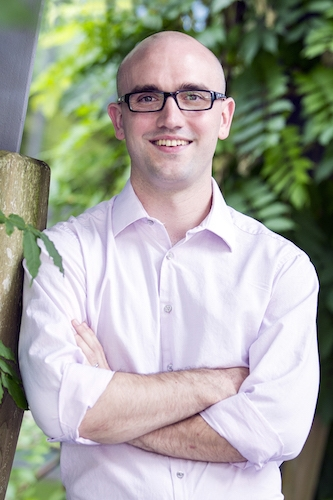
\includegraphics[height=2.5cm]{scott-seas_0}
	\caption{Scott Kuindersma}
	\end{subfigure}%
	\begin{subfigure}{.5\textwidth}
	\centering
	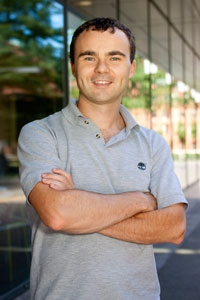
\includegraphics[height=2.5cm]{walsh_200x300}
	\caption{Conor Walsh}
	\end{subfigure}%
	\end{figure}

	\begin{figure}
	\captionsetup[subfigure]{labelformat=empty}
	\begin{subfigure}{.3\textwidth}
	\centering
	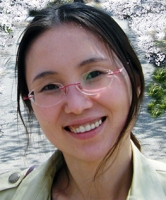
\includegraphics[height=2.5cm]{kim_myunghee}
	\caption{Myunghee Kim}
	\end{subfigure}%
	\begin{subfigure}{.3\textwidth}
	\centering
	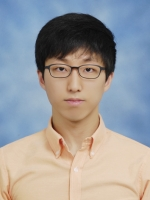
\includegraphics[height=2.5cm]{kim_jinsoo}
	\caption{Jinsoo Kim}
	\end{subfigure}%
	\begin{subfigure}{.3\textwidth}
	\centering
	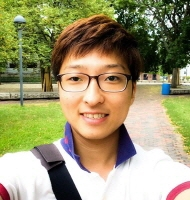
\includegraphics[height=2.5cm]{sangjun}
	\caption{Sangjun Lee}
	\end{subfigure}%
	\end{figure}
\end{frame}

\begin{comment}
\begin{frame}
\frametitle{\textbf{Include a graphic}}
\begin{figure}[htb]
\spacingset{1}
\centerline{\includegraphics[scale=.40]{data/postprocessing/AvatarSelectionPlot-Role2.pdf}}
\end{figure}
\end{frame}
\end{comment}


%this way you can have a bibliography in your slides.
%\begin{comment}
%\begin{frame}[allowframebreaks]
%\def\newblock{}
%\bibliography{TingleyBib}
%\end{frame}
%\end{comment}



\end{document}